\chapter{Finite Element Formulation}\label{chap:fem}
\section{Weak formulation}
The final equation obtained by applying various thermodynamic properties are following
\begin{eqnarray}
-\nabla \cdot u &=& \frac{1}{p^0} \frac{d p^0}{d t} - \frac{1}{T}\frac{D T}{D t} \hspace{1mm}\\
\rho \frac{D u}{D t} \hspace{1mm} &=& -\frac{1}{M^2}\hspace{1mm}\nabla p\hspace{1mm}+\hspace{1mm}\frac{1}{Re}\nabla \cdot (\mu (\nabla u +(\nabla u)^T) - \frac{2}{3}\mu \nabla \cdot u I) + \frac{1}{Fr^2}\rho g \\
\rho C_p \frac{D T}{D t} \hspace{1mm}&=&\hspace{1mm} -  \frac{1}{Re Pr}\nabla\cdot (k \nabla T) + \hspace{1mm} \frac{1}{\gamma -1} \frac{d p^0}{d t}\hspace{1mm}\\
\end{eqnarray}
The 2D finite element weak form  is given as

\begin{eqnarray*}
\int_{0}^{L} \int_{0}^{L}\rho \frac{\partial u^h}{\partial t} \psi + \hspace{1mm}\int_{0}^{L} \int_{0}^{L} (\rho u^h \cdot \nabla u^h ) \psi \hspace{1mm} &=& \int_{0}^{L} \int_{0}^{L}  -\frac{1}{M^2}\hspace{1mm}(\nabla p^h) \phi \hspace{1mm}+\hspace{1mm}\int_{0}^{L} \int_{0}^{L}\frac{1}{Re}(\nabla \cdot \tau^h) \psi+ \\ \int_{0}^{L} \int_{0}^{L}\frac{1}{Fr^2}(\rho g )\psi \\
\int_{0}^{L} \int_{0}^{L} \rho C_p \frac{\partial T^h}{\partial t} \varphi + \hspace{1mm}\int_{0}^{L} \int_{0}^{L} \rho C_p (u^h \cdot \nabla T^h ) \varphi  \hspace{1mm}&=&\hspace{1mm} \int_{0}^{L} \int_{0}^{L} -  \frac{1}{Re Pr}(\nabla\cdot k \nabla T^h) \varphi  + \int_{0}^{L} \int_{0}^{L} \hspace{1mm} \frac{1}{\gamma -1} \frac{d p^h}{d t} \phi  \hspace{1mm}\\
\end{eqnarray*}

Integrating by parts and applying boundary conditions

\begin{eqnarray*}
\int_{0}^{L} \int_{0}^{L}\rho \dot{u}^h \psi_i \psi_j + \hspace{1mm}\int_{0}^{L} \int_{0}^{L} \rho u^h \cdot \nabla u^h \psi_i \hspace{1mm} &=& \int_{0}^{L} \int_{0}^{L}  -\frac{1}{M^2}\hspace{1mm}\nabla p^h \phi_i \hspace{1mm} - \hspace{1mm}\int_{0}^{L} \int_{0}^{L}\frac{1}{Re} \tau^h \nabla \psi + \left[\tau \psi \right]_0^L+ \\ \int_{0}^{L} \int_{0}^{L}\frac{1}{Fr^2}\rho g \psi \\
\int_{0}^{L} \int_{0}^{L} \rho C_p \dot{T}^h \varphi_i \varphi_j + \hspace{1mm}\int_{0}^{L} \int_{0}^{L} \rho C_p u^h \cdot \nabla T \varphi_i \hspace{1mm}&=&\hspace{1mm} \int_{0}^{L} \int_{0}^{L} +  \frac{1}{Re Pr}(k \nabla T^h) \nabla \varphi  -  \frac{1}{Re Pr} \left[k \nabla T^h \varphi \right]_0^L \\ + \int_{0}^{L} \int_{0}^{L} \hspace{1mm} \frac{1}{\gamma -1} \frac{d p^h}{d t} \phi\hspace{1mm} \\
\end{eqnarray*}

\section{Need for stability}
Using numerical methods in a straightforward way for the approximation of arbitrary differential
equations may cause severe problems. There are Oscillations, locking, singular matrices and other problems in the result in certain concrete problem.
Thus, stabilization is needed. To obtain satisfactory approximations stabilization may be needed. The matrix of the advective term is non-symmetric (non-self adjointness of the convective operator) and the ”best approximation” property is lost . As a result Bubnov-Galerkin methods applied to these problems are far from ”optimal” and show spurious oscillations in the solutions, worsening with growing convection-domination. 

 To characterize the relative importance of convective and diffusive effects in a given flow
problem, it is useful to introduce the mesh Peclet number.

$$Pe=\frac{ah}{2\nu}$$

 which expresses the ratio of convective to diffusive transport.
The  Galerkin solution is corrupted by non-physical oscillations when the Peclet number is larger than one. The Galerkin method loses its best approximation property when the non-symmetric convection operator dominates the diffusion operator in the transport equation, and consequently spurious node-to-node oscillations appear.

 All stabilization schemes applied are Petrov-Galerkin approaches. They all add perturbations to the original Bubnov-Galerkin weak form. These perturbations are formulated in terms of modifications of the Bubnov-Galerkin test functions. They are multiplied with the residuals of the differential equations and thereby ensure consistency. Additionally, a stabilization parameter $\xi$ weights the influence of the added stabilization terms.

\subsection{Streamline Upwind Petrov Galerkin Method}
To ensure that the solution of the differential equation is also a solution of the
weak form, it is necessary to stabilize the convective term in a consistent manner. To accomplish this an extra term over the element interiors is added
to the Galerkin weak form. This term has to be a function of the residual of the differential equation or else the equation will not be consistent. It introduces a certain amount of artificial diffusion in streamline direction only. The latter aspect ensures that no diffusion perpendicular to the flow direction is introduced, which was the reason for excessive over diffusion in other methods. 

\bigskip
 Stabilization through a product of a perturbation and the residual
is a fundamental aspect of successful stabilization schemes and is realized in all stabilization method
applied here. The following term is added to the galerkin weak form of the differential equation. 

 $$\sum_e \int_{\Omega^e} P(w) \xi R(u)  d\Omega$$ 


\bigskip
 Where $P(w)$ is a certain operator applied to the test function, $\xi$ is the stabilization
parameter (also called intrinsic time), and $R(u)$ is the residual of the differential
equation. The stabilization techniques are characterized by the definition of $P(w)$

\bigskip
 The SUPG stabilization technique is defined by taking


$$P(w)= a.\nabla w$$  where a is the convection velocity. $w$ is the test function.  This corresponds to the perturbation of the test function. The space of the test functions does not coincide with the space of the interpolation functions, hence it is called as Petrov—Galerkin formulation.

 For simple convection diffusion equation
\bigskip
 $\tau = \frac{\overrightarrow{\nu}}{\vert \vert a \vert\vert^2}$. For 1D $\overrightarrow{\nu}=\frac{\beta a h}{2}$ and $\beta = coth(Pe)-\frac{1}{Pe}$
 
 \subsection{Pressure-Stabilizing/Petrov-Galerkin (PSPG)} 
 
 In mixed convection-dominated problems, such as the incompressible Navier-Stokes equations
 with high Reynolds-numbers, SUPG and PSPG (called herein SUPG/PSPG) stabilization have to
 be applied to obtain satisfactory results. It should also be mentioned that the PSPG stabilization parameter does not necessarily have to be identical with the SUPG stabilization parameter
 
 \bigskip
  The terms associated with parameter $\xi_{pspg}$ (pressure-stabilizing/Petrov-Galerkin)
 allow the use of mixed elements with equal-order interpolations for the velocity and
 pressure. All stabilization
 terms are weighted residuals, therefore ensuring the consistency of the formulation. The following term is added to the galerkin weak form of the differential equation. 
 
  $$\sum_e \int_{\Omega^e} \nabla \phi \xi_{pspg} R(u)  d\Omega$$ 
 
 \subsection{Stabilized Navier Stokes Equation} 
 From the stabilization discussions we can now write the stabilized form of Navier stokes equation. The Residual of momentum and energy equation are given as follows
\bigskip
\begin{eqnarray*}
R1(u) &=& \rho \frac{D u^h}{D t} \hspace{1mm} + \frac{1}{M^2}\hspace{1mm}\nabla p^h\hspace{1mm}-\hspace{1mm}\frac{1}{Re}\nabla \cdot (\mu^*(\nabla u^h +(\nabla u^h)^T) - \frac{2}{3}\mu^h \nabla \cdot u^h I) - \frac{1}{Fr^2}\rho g \\
R2(T) &=& \rho C_p \frac{D T^h}{D t} \hspace{1mm} \hspace{1mm} + \frac{1}{Re Pr}\nabla\cdot (k \nabla T^h) - \hspace{1mm} \frac{1}{\gamma -1} \frac{d p^h}{d t}\hspace{1mm}
\end{eqnarray*}

\bigskip
 Now adding the pressure stabilization and convection stabilization to momentum and energy equations we get the following expressions
\begin{eqnarray*}
\int_{0}^{L} \int_{0}^{L}\rho \dot{u}^h \psi_i \psi_j + \hspace{1mm}\int_{0}^{L} \int_{0}^{L} \rho u^h \cdot \nabla u^h \psi_i \hspace{1mm}  + \int_{0}^{L} \int_{0}^{L}  \frac{1}{M^2}\hspace{1mm}\nabla p^h \phi_i \hspace{1mm} + \hspace{1mm}\int_{0}^{L} \int_{0}^{L}\frac{1}{Re} \tau^h \nabla \psi +  \\ - \int_{0}^{L} \int_{0}^{L}\frac{1}{Fr^2}\rho g \psi + \sum_e \int_{\Omega^e} P(\psi) \xi R1(u)  d\Omega + \sum_e \int_{\Omega^e} \nabla \phi \xi_{pspg} R1(u)  d\Omega  &=& \left[\tau \psi \right]_0^L \\
\int_{0}^{L} \int_{0}^{L} \rho C_p \dot{T}^h \varphi_i \varphi_j + \hspace{1mm}\int_{0}^{L} \int_{0}^{L} \rho C_p u^h \cdot \nabla T \varphi_i \hspace{1mm} - \hspace{1mm} \int_{0}^{L} \int_{0}^{L} \frac{1}{Re Pr}(k \nabla T^h) \nabla \varphi - \\ \int_{0}^{L} \int_{0}^{L} \hspace{1mm} \frac{1}{\gamma -1} \frac{d p^h}{d t} \phi +  \sum_e \int_{\Omega^e} S(\varphi) \xi R2(T)  d\Omega + \sum_e \int_{\Omega^e} \nabla \varphi \xi_{pspg} R2(T)  d\Omega &=& -  \frac{1}{Re Pr} \left[k \nabla T^h \varphi \right]_0^L \hspace{1mm}\\
\end{eqnarray*}


\section{Adaptive Finite Element}


\section{Geometry with boundary conditions}

\begin{figure}[H]
  
  \centering
   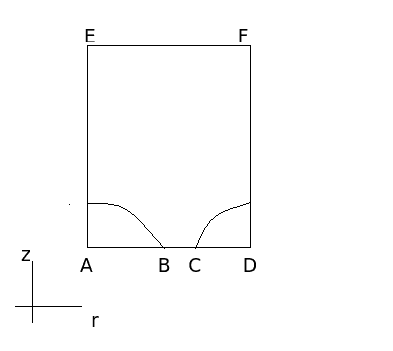
\includegraphics[scale=0.5]{figs/geometricbcs}
   \caption{Geometry}
\end{figure}
\begin{itemize}
\item $AB$ is the inlet
\item $BC$ is the thickness of the burner tube
\item $CD$ is the outside of the burner
\item $DE,EF$ is the domain of interest
\item $AE$ is the Axisymmetric line
\end{itemize}

\bigskip
 The following assumption are made
\begin{itemize}
\item At the inlet, the incoming velcity has parabolic profile. i.e poissuelle flow. 
\item The surface chemistry at the wall of the burner is neglected. 
\item At the outside of the burner, the incoming air has couette flow profile. 
\item $DE,EF$ are the boundaries of the domain. No change occurs after this point. 
\end{itemize}
	
 The boundary conditions are defined as follows 
\bigskip

 At the inlet ($AB$)
\begin{itemize}
\item $u_r = 0$ and $u_z=5801.9 mm/s$
\item $C_i = 1$ 
\item $T = 300K$
\item $p=1 atmos$
\end{itemize}

\bigskip 
 On $BC$
\begin{itemize}
\item $u_r = 0$ and $u_z=0 mm/s$
\item $\frac{\partial C_i}{\partial r} =0 $ and $\frac{\partial C_i}{\partial z} =0 $
\item $T = 300K$
\item $p=1 atmos$
\end{itemize}

 On $CD$
\begin{itemize}
\item $u_r = 0$ and $u_z=5801.9 mm/s$
\item $ C_{O_2} =21 \% $
\item $T = 300K$
\item $p=1 atmos$
\end{itemize}

 On $DF$ and $FE$
\begin{itemize}
\item $\frac{\partial u_r}{\partial r} =0 $ and $\frac{\partial u_z}{\partial z} =0 $
\item $\frac{\partial C_i}{\partial r} =0 $ and $\frac{\partial C_i}{\partial z} =0 $
\item $\frac{\partial T}{\partial r} =0 $ and $\frac{\partial T}{\partial z} =0 $
\item $\frac{\partial p}{\partial r} =0 $ and $\frac{\partial p}{\partial z} =0 $
\end{itemize}


 On $AF$
\begin{itemize}
\item $\frac{\partial u_r}{\partial r} =0 $ 
\item $\frac{\partial C_i}{\partial r} =0 $ 
\item $\frac{\partial T}{\partial r} =0 $  
\item $\frac{\partial p}{\partial r} =0 $
\end{itemize}


